\documentclass{article}
\usepackage{geometry}
\usepackage{fancyhdr}
\usepackage{amsmath ,amsthm ,amssymb}
\usepackage{graphicx}
\usepackage{hyperref}
\usepackage{comment}
\usepackage{csvsimple}


\begin{document}

\begin{titlepage}

\newcommand{\HRule}{\rule{\linewidth}{0.5mm}} % Defines a new command for the horizontal lines, change thickness here

\center % Center everything on the page
 
%----------------------------------------------------------------------------------------
%	HEADING SECTIONS
%----------------------------------------------------------------------------------------

%\textsc{\LARGE National University of Singapore}\\[1.5cm] % Name of your university/college
%\textsc{\large Minor Heading}\\[0.5cm] % Minor heading such as course title

%----------------------------------------------------------------------------------------
%	TITLE SECTION
%----------------------------------------------------------------------------------------

\HRule \\[0.4cm]
{ \huge \bfseries CS5340 Project Report}\\[0.4cm] % Title of your document
\HRule \\[1.5cm]


%----------------------------------------------------------------------------------------
%	AUTHOR SECTION
%----------------------------------------------------------------------------------------


% If you don't want a supervisor, uncomment the two lines below and remove the section above
\Large \emph{By:}\\
Neha Priyadarshini Garg (A0117042W)\\ % Your name
Xin Yi (A0142487Y)\\
Zhu Lei (A0105790H)\\[3cm]

%----------------------------------------------------------------------------------------
%	DATE SECTION
%----------------------------------------------------------------------------------------

{\large \today}\\[2cm] % Date, change the \today to a set date if you want to be precise

\vfill % Fill the rest of the page with whitespace

\end{titlepage}

\bibliographystyle{apalike}

%\title{Learning and Planning for Autonomous Grasping in Uncontrolled Environments}
%\author{Neha Priyadarshini Garg}
%\maketitle


\section{Problem 1 : Data Denoising}
\subsection{Potential function}
For data denoising using Gibbs Sampling, we used the following pairwise potential term:\\
\begin{equation}
\psi_t(x_t, x_s) = e^{J*x_t*x_s}
\end{equation}
Where $J$ is a constant parameter which can control the influence of neighboring pixels on the current pixel. Setting J = 3 gave us good results as can be seen in section \ref{results_1}.

For local evidence, we used gaussian distribution with mean as the original pixel value and variance as $sqrt(1/2)$. Thus we defined local evidence as follows:
\begin{equation}
\psi_t(x_t) = e^{-(x_t - y_t)^2}
\end{equation}

\subsection{Algorithm}
Using these potential functions, we could calculate $p(x_t=1| x_{-t},y,\theta)$ as follows:
\begin{equation}
p(x_t=1| x_{-t},y,\theta) = \frac{\psi_t(x_t=1)\Pi_{s \in nbr(t)}\psi_t(x_t=1, x_s)}{\psi_t(x_t=1)\Pi_{s \in nbr(t)}\psi_t(x_t=1, x_s) + \psi_t(x_t=-1)\Pi_{s \in nbr(t)}\psi_t(x_t=-1, x_s)}
\end{equation}


Using the above probability distribution for each pixel, we did gibbs sampling with 1100 iterations out of which first 100 iterations were set as burn-in.

\subsection{Results}

\label{results_1}

\begin{center}
 \begin{tabular}{||c c||}
 \hline

 \includegraphics[width=.4\linewidth]{../../a1/1_noise.png} & 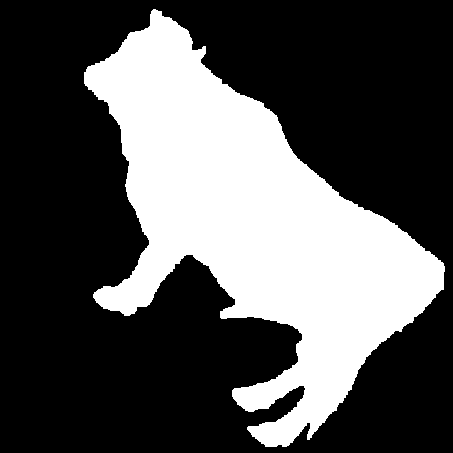
\includegraphics[width=.4\linewidth]{../image-denoising/output/1_denoise.png} \\ 
 \hline
 \end{tabular}
\end{center}

\begin{center}
 \begin{tabular}{||c c||}
 \hline
 \includegraphics[width=.4\linewidth]{../../a1/2_noise.png} & 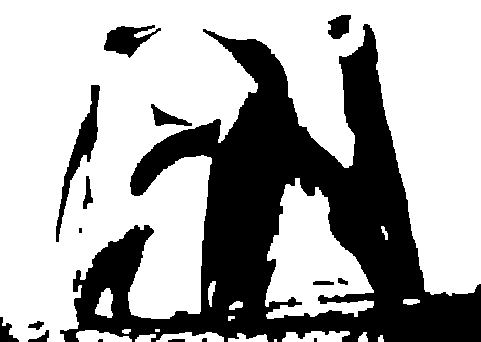
\includegraphics[width=.4\linewidth]{../image-denoising/output/2_denoise.png} \\ 
 \hline
  \end{tabular}
\end{center}

\begin{center}
 \begin{tabular}{||c c||}
 \hline
 \includegraphics[width=.4\linewidth]{../../a1/3_noise.png} & 
\includegraphics[width=.4\linewidth]{../image-denoising/output/3_denoise.png} \\ 
 \hline
  \end{tabular}
\end{center}

\begin{center}
 \begin{tabular}{||c c||}
 \hline
 \includegraphics[width=.4\linewidth]{../../a1/4_noise.png} & 
\includegraphics[width=.4\linewidth]{../image-denoising/output/4_denoise.png} \\ 
 \hline

\end{tabular}
\end{center}


\section{Problem 2 : Expectation-Maximization Segmentation}
\subsection{Features}
We tried 3 different features for image segmentation.\\
1) Lab features : The L, a and b values for each pixel \\
2) Lab features with neighbour difference : For each pixel, we sum the differences of its L, a and b values with its neighbours' to form three new features for that pixel. \\
3) Lab features with avg neighbour : For each pixel, we average its L, a and b values and its neighbours to form three new features for that pixel. \\

From the results, we can see that Lab features with avg neighbour perform better that just Lab features as with the help of neighbours, small noise is filtered out more efficiently. However in case of zebra, this leads to worse results as white stripes of zebra are also filtered out. This shows the importance of correctly defining features.

\subsection{Algorithm}
For a given feature set, we first initialize the mean and covariance parameters of 2 gaussians by setting the covariance as covariance of the features for whole image and mean as a random value which is not very far from the actual mean for the whole image.

Then we calculate the probabilities for all pixels belonging to a given segments using gaussian functions as described in problem definition. Then we update parameters of gaussians by calculating weighted mean and covariances using probabilities calculated in E-step as weights. We update the mixing parameters by summing up the probabilities for each segment. We do this iteratively until the change in parameters is very small.

\subsection{Results}

\begin{center}
\begin{tabular}{c}
\includegraphics[width=.4\linewidth]{../../a2/cow.jpg}
\end{tabular}
\\
\begin{tabular}{c}

Lab Features \\
\end{tabular}
 \begin{tabular}{c c c} 

 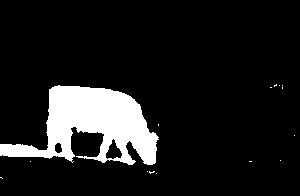
\includegraphics[width=.4\linewidth]{../image-segmentation/output/Lab/cow_mask.jpg} & 
 
 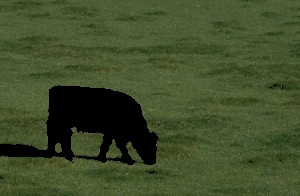
\includegraphics[width=.4\linewidth]{../image-segmentation/output/Lab/cow_seg1.jpg} & 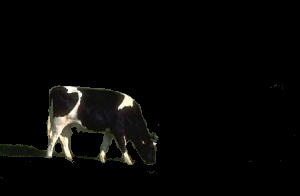
\includegraphics[width=.4\linewidth]{../image-segmentation/output/Lab/cow_seg2.jpg} \\
  
 \end{tabular}
 \begin{tabular}{c}

Lab features with neighbour difference \\
\end{tabular}
 \begin{tabular}{c c c} 

 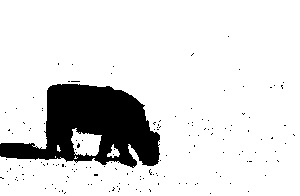
\includegraphics[width=.4\linewidth]{../image-segmentation/output/add-Lab-neighbor-diff-feature/cow_mask.jpg} & 
 
 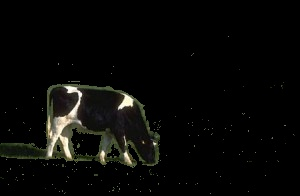
\includegraphics[width=.4\linewidth]{../image-segmentation/output/add-Lab-neighbor-diff-feature/cow_seg1.jpg} & 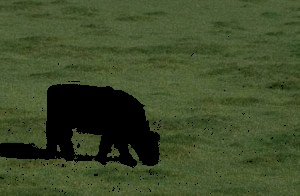
\includegraphics[width=.4\linewidth]{../image-segmentation/output/add-Lab-neighbor-diff-feature/cow_seg2.jpg} \\
  
 \end{tabular}
 \begin{tabular}{c}

Lab features with avg neighbour \\
\end{tabular}
 \begin{tabular}{c c c} 

 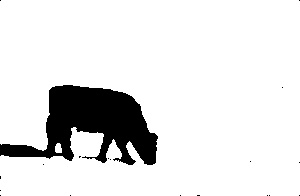
\includegraphics[width=.4\linewidth]{../image-segmentation/output/add-Lab-neighbor-avg-feature/cow_mask.jpg} & 
 
 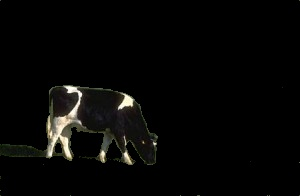
\includegraphics[width=.4\linewidth]{../image-segmentation/output/add-Lab-neighbor-avg-feature/cow_seg1.jpg} & 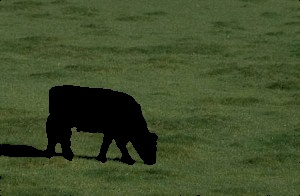
\includegraphics[width=.4\linewidth]{../image-segmentation/output/add-Lab-neighbor-avg-feature/cow_seg2.jpg} \\
  
 \end{tabular}
 
 
\end{center}



\begin{center}
\begin{tabular}{c}
\includegraphics[width=.4\linewidth]{../../a2/owl.jpg}
\end{tabular}
\\
\begin{tabular}{c}

Lab Features \\
\end{tabular}
 \begin{tabular}{c c c} 

 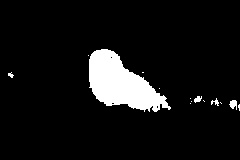
\includegraphics[width=.4\linewidth]{../image-segmentation/output/Lab/owl_mask.jpg} & 
 
 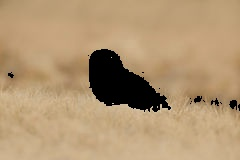
\includegraphics[width=.4\linewidth]{../image-segmentation/output/Lab/owl_seg1.jpg} & 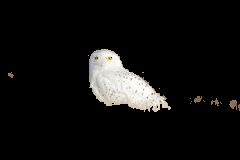
\includegraphics[width=.4\linewidth]{../image-segmentation/output/Lab/owl_seg2.jpg} \\
  
 \end{tabular}
 \begin{tabular}{c}

Lab features with neighbour difference \\
\end{tabular}
 \begin{tabular}{c c c} 

 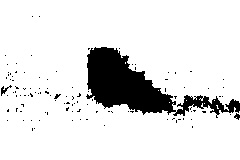
\includegraphics[width=.4\linewidth]{../image-segmentation/output/add-Lab-neighbor-diff-feature/owl_mask.jpg} & 
 
 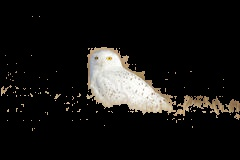
\includegraphics[width=.4\linewidth]{../image-segmentation/output/add-Lab-neighbor-diff-feature/owl_seg1.jpg} & 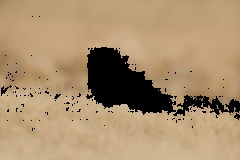
\includegraphics[width=.4\linewidth]{../image-segmentation/output/add-Lab-neighbor-diff-feature/owl_seg2.jpg} \\
  
 \end{tabular}
 \begin{tabular}{c}

Lab features with avg neighbour \\
\end{tabular}
 \begin{tabular}{c c c} 

 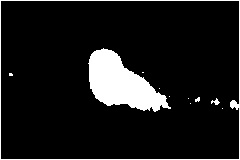
\includegraphics[width=.4\linewidth]{../image-segmentation/output/add-Lab-neighbor-avg-feature/owl_mask.jpg} & 
 
 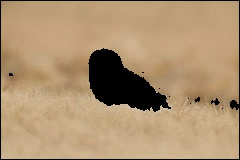
\includegraphics[width=.4\linewidth]{../image-segmentation/output/add-Lab-neighbor-avg-feature/owl_seg1.jpg} & 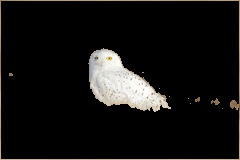
\includegraphics[width=.4\linewidth]{../image-segmentation/output/add-Lab-neighbor-avg-feature/owl_seg2.jpg} \\
  
 \end{tabular}
 
 
\end{center}





\begin{center}
\begin{tabular}{c}
\includegraphics[width=.4\linewidth]{../../a2/fox.jpg}
\end{tabular}
\\
\begin{tabular}{c}

Lab Features \\
\end{tabular}
 \begin{tabular}{c c c} 

 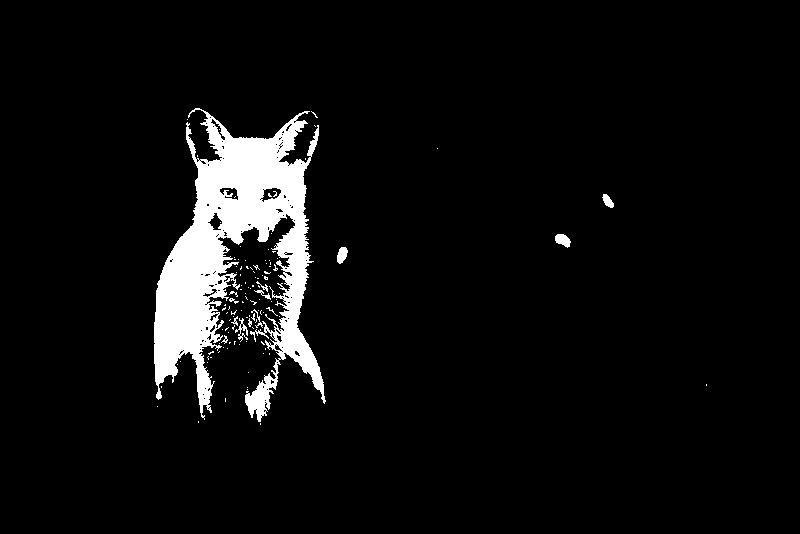
\includegraphics[width=.4\linewidth]{../image-segmentation/output/Lab/fox_mask.jpg} & 
 
 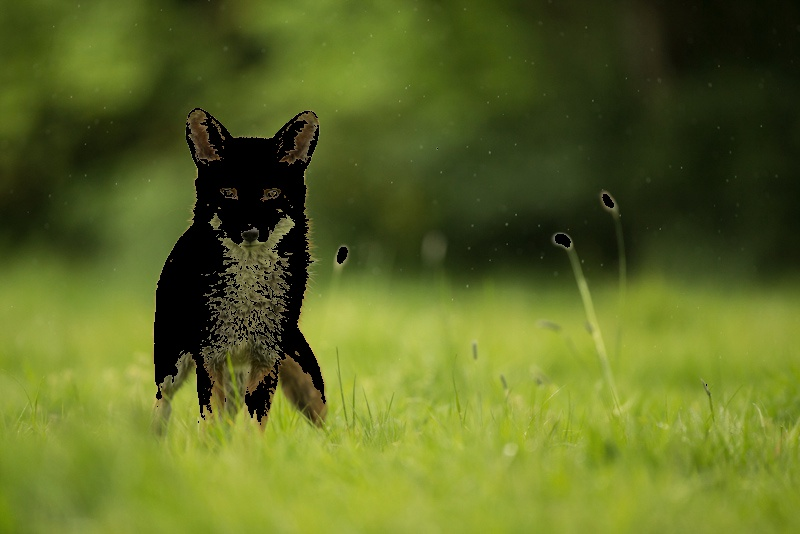
\includegraphics[width=.4\linewidth]{../image-segmentation/output/Lab/fox_seg1.jpg} & 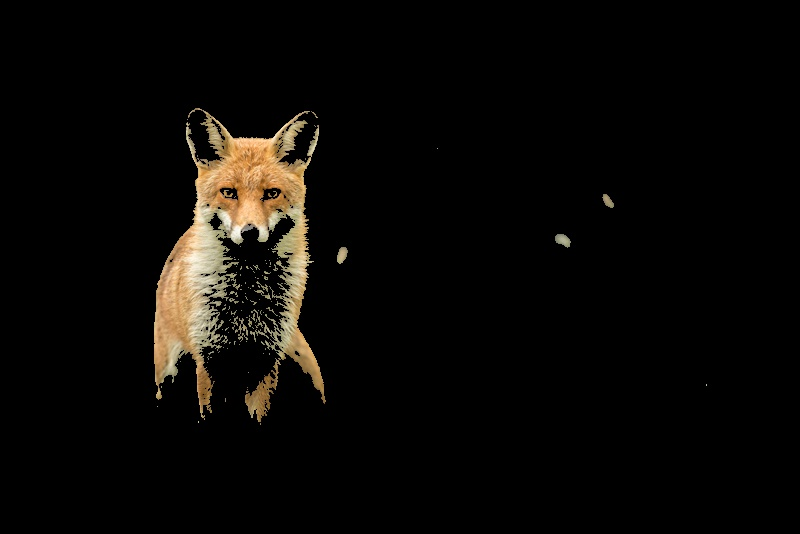
\includegraphics[width=.4\linewidth]{../image-segmentation/output/Lab/fox_seg2.jpg} \\
  
 \end{tabular}
 \begin{tabular}{c}

Lab features with neighbour difference \\
\end{tabular}
 \begin{tabular}{c c c} 

 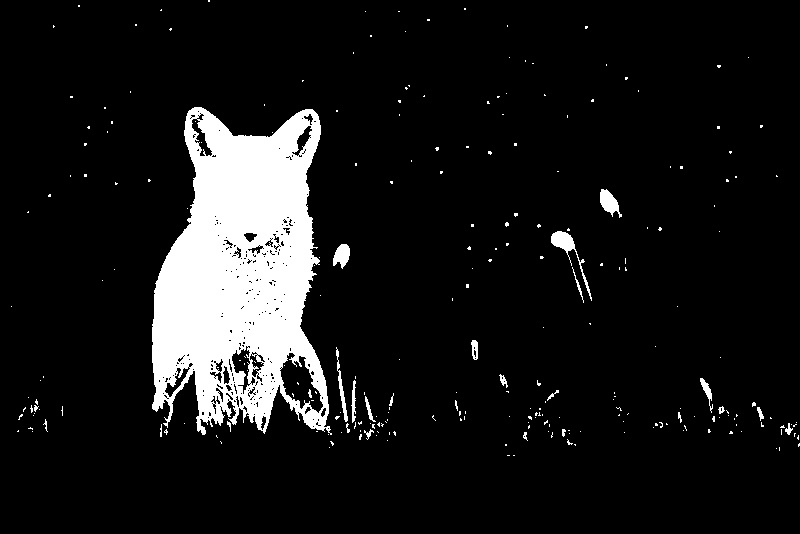
\includegraphics[width=.4\linewidth]{../image-segmentation/output/add-Lab-neighbor-diff-feature/fox_mask.jpg} & 
 
 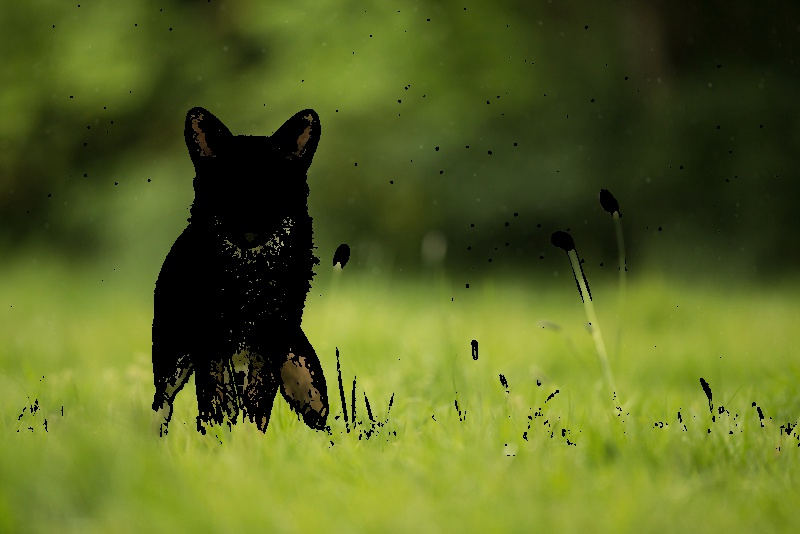
\includegraphics[width=.4\linewidth]{../image-segmentation/output/add-Lab-neighbor-diff-feature/fox_seg1.jpg} & 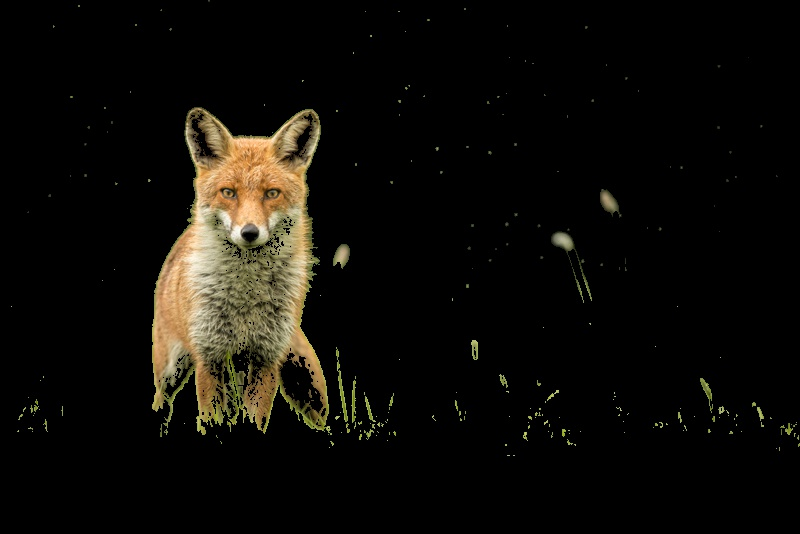
\includegraphics[width=.4\linewidth]{../image-segmentation/output/add-Lab-neighbor-diff-feature/fox_seg2.jpg} \\
  
 \end{tabular}
 \begin{tabular}{c}

Lab features with avg neighbour \\
\end{tabular}
 \begin{tabular}{c c c} 

 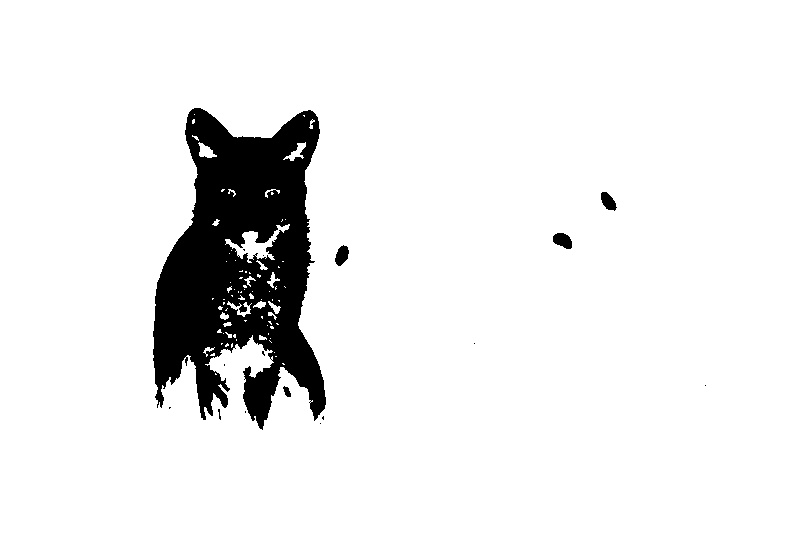
\includegraphics[width=.4\linewidth]{../image-segmentation/output/add-Lab-neighbor-avg-feature/fox_mask.jpg} & 
 
 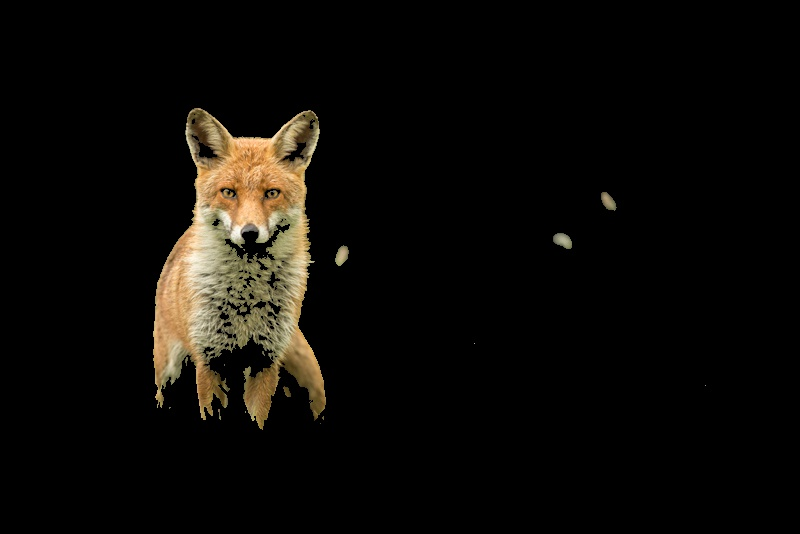
\includegraphics[width=.4\linewidth]{../image-segmentation/output/add-Lab-neighbor-avg-feature/fox_seg1.jpg} & 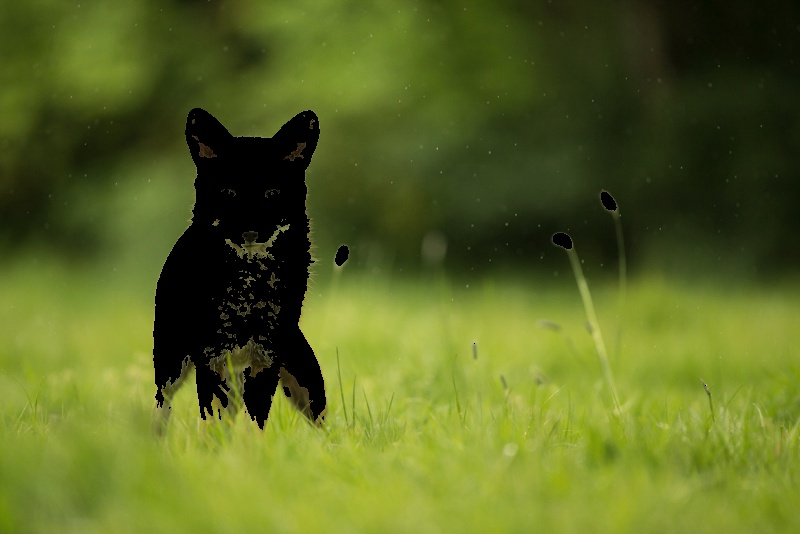
\includegraphics[width=.4\linewidth]{../image-segmentation/output/add-Lab-neighbor-avg-feature/fox_seg2.jpg} \\
  
 \end{tabular}
 
 
\end{center}


\begin{center}
\begin{tabular}{c}
\includegraphics[width=.4\linewidth]{../../a2/zebra.jpg}
\end{tabular}
\\
\begin{tabular}{c}

Lab Features \\
\end{tabular}
 \begin{tabular}{c c c} 

 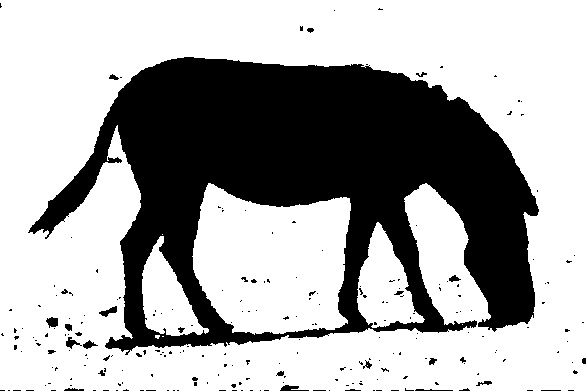
\includegraphics[width=.4\linewidth]{../image-segmentation/output/Lab/zebra_mask.jpg} & 
 
 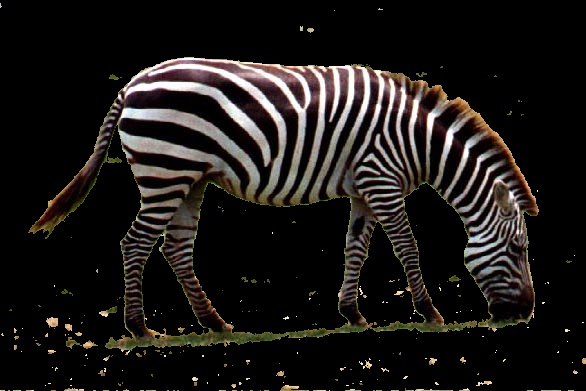
\includegraphics[width=.4\linewidth]{../image-segmentation/output/Lab/zebra_seg1.jpg} & 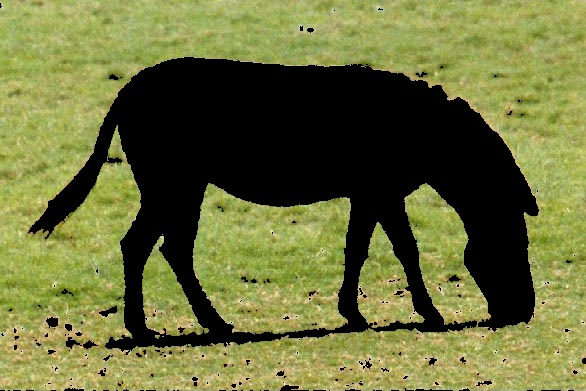
\includegraphics[width=.4\linewidth]{../image-segmentation/output/Lab/zebra_seg2.jpg} \\
  
 \end{tabular}
 \begin{tabular}{c}

Lab features with neighbour difference \\
\end{tabular}
 \begin{tabular}{c c c} 

 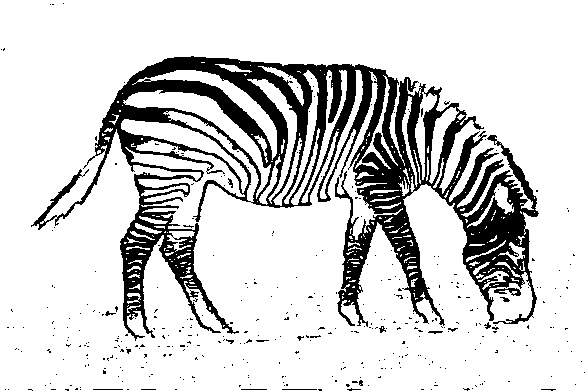
\includegraphics[width=.4\linewidth]{../image-segmentation/output/add-Lab-neighbor-diff-feature/zebra_mask.jpg} & 
 
 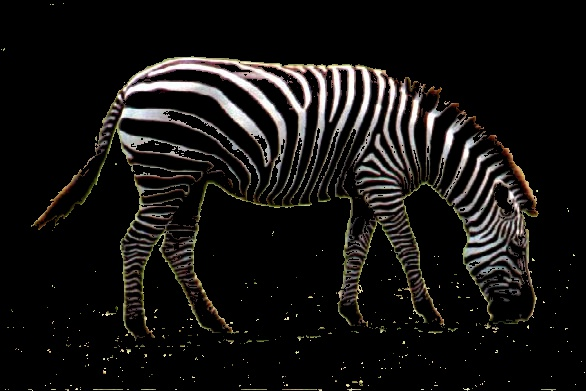
\includegraphics[width=.4\linewidth]{../image-segmentation/output/add-Lab-neighbor-diff-feature/zebra_seg1.jpg} & 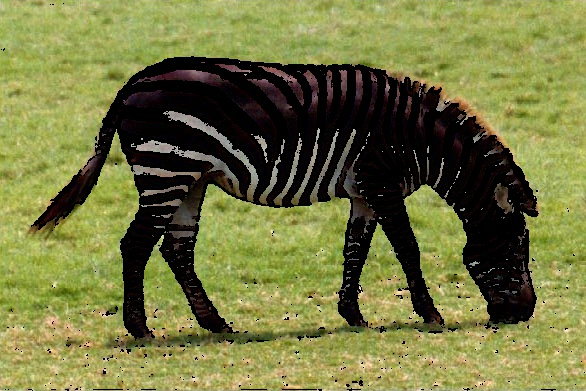
\includegraphics[width=.4\linewidth]{../image-segmentation/output/add-Lab-neighbor-diff-feature/zebra_seg2.jpg} \\
  
 \end{tabular}
 \begin{tabular}{c}

Lab features with avg neighbour \\
\end{tabular}
 \begin{tabular}{c c c} 

 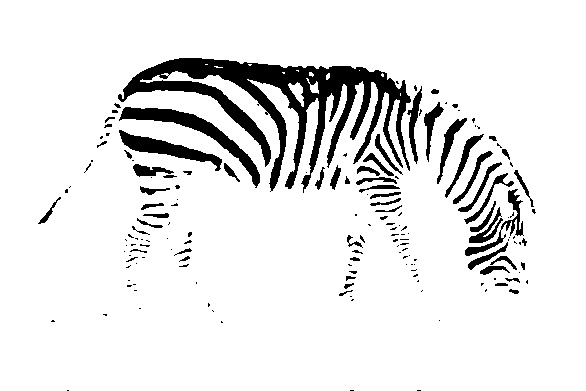
\includegraphics[width=.4\linewidth]{../image-segmentation/output/add-Lab-neighbor-avg-feature/zebra_mask.jpg} & 
 
 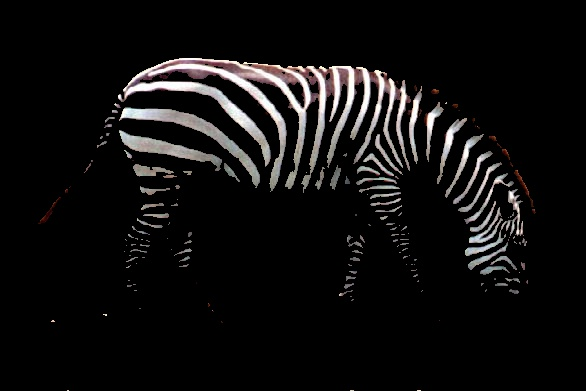
\includegraphics[width=.4\linewidth]{../image-segmentation/output/add-Lab-neighbor-avg-feature/zebra_seg1.jpg} & 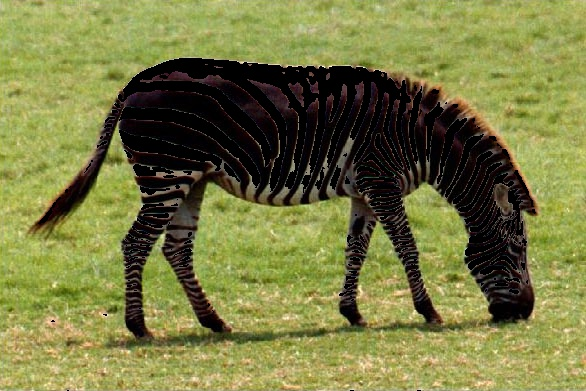
\includegraphics[width=.4\linewidth]{../image-segmentation/output/add-Lab-neighbor-avg-feature/zebra_seg2.jpg} \\
  
 \end{tabular}
 
 
\end{center}




%\bibliography{relatedWork}


\end{document}
